%================================================================
%                           N O T E S
%                           ---------
%
%                           ---------
%-----------------------------------------------------------------
%                       INTRODUCTION
%-----------------------------------------------------------------
\section{Introduction}
%
The goal of this tool was to plot the scattered field. I took Prof. Guettel's Introduction to Python in 2nd Year and was interested in learning more about using the language.

I started off with a text file on my laptop but quickly realised I would benefit from version controlling it, so I created a repository on Bitbucket. It can be accessed \href{https://bitbucket.org/veracruz/canonical_scattering}{here}. It also helped me version control this document, since it became quite complex quickly.

In Prof. Guettel's introduction to Python we exclusively used functions to build a game of Othello that ran in the command line. This is very different to what I have done here, where I would need the programme to output the file of the plotted field. Additionally, this tool became many orders of magnitude more complex because of the nature of the problem and I thought it appropriate to employ an object oriented approach.

%-----------------------------------------------------------------
%                       THE SET UP
%-----------------------------------------------------------------
\section{Approach}

My tool went through a lot of different verisons but in it's final state it is comprised of four python files and one json file. The json file was a late addition which made it much easier to set and carry over values for variables, which originally had to be set for every particular wave instantiation.

The json file is called \verb!data.txt! and is not very complex:
\begin{lstlisting}
{
  "axis_length" : [int],
  "axis_delta" : [int],
  "truncation" : [int],
  "wavevector" : [[float], [float]],
  "cylinder_radius" : [float],
  "speed_of_sound" : 343,
  "boundary_type" : [str],
  "field_type" : [str],
  "density_inside" : [float],
  "density_outside" : [float]
} \end{lstlisting}
however this data needs to be brought into the tool. For this I created the \verb!inputs.py! file, which holds the \verb!Inputs! class. This class is then fed through to all other classes so all the variables throughout the tool are set by the \verb!data.txt! file. This was a big change from having the variables be determined independently at different points in the plotting process, and helps protect the methods when changing what function to plot.

The \verb!plotter.py! file holds two classes: \verb!Main! and \verb!Wave!. The \verb!Main! class is used ot run the programme itself, and the \verb!Wave! class holds all the functions that are common to all wave instantiations. The \verb!fields.py! file holds subclasses which are instantiations of the \verb!Wave! class. Finally we have the \verb!grpahics.py! file which holds the \verb!Graphics! class where the plots are created.

Within the \verb!Main! class I defined the \verb!run! class, which runs the tool when it is compiled as a python script from the command line. I also define different functions for different fields I want to plot in this class, so that it is easy to call them. For example, for the cylinder scattering problem I call

  \begin{lstlisting}
self.create_field_around_cylinder(self.graph) \end{lstlisting}
where I have defined
  \begin{lstlisting}
def create_field_around_cylinder(self, graph):
    field = CylinderField()
    graph.heat_map(field) \end{lstlisting}
and \verb!self.graph = Graphics! was set within the \verb!__init__! constructor method.


%-----------------------------------------------------------------
%                        INPUTS CLASS
%-----------------------------------------------------------------

\subsection{}ection{The \texttt{Inputs} class}

The \verb!Inputs! class has two objectives, to read the \verb!data.txt! file and to create local variables that can be passed through to the other classes. These variables are either read directly from the file or calculated. The \verb!read_file! method returns a dictionary containing all the data in the json file.

\begin{lstlisting}
def read_file(self):
    file = open(r"data.txt", "r")
    return json.load(file)\end{lstlisting}

This is then used in the \verb!set_params! function to set the local variables directly from the file.

The \verb!data.txt! file was originally read as a \verb!csv! file instead of \verb!json!. This became cumbersome very quickly though, since \verb!csv! are read line by line. The only way to tell the reader which bit of information to pass through is to point at a line and position which is prone to human error. In contrast \verb!json! has named variables, which makes it easier to reference.

Since all the information in \verb!data.txt! is inputted manually I decided to make sure to do add error messages at this stage, so that if I have inputted the wrong variable type it will be caught immediately and won't cause bugs that would be hard to pinpoint later on. If there is an error.

\begin{lstlisting}
def set_params(self):
    dict = self.read_file()

    ## TYPE OF BCS
    self.boundary_type = dict['boundary_type']

    ## FIELD TYPE
    self.field_type = dict['field_type']

    [...]

    ##  TRUNCATION
    try:
        self.truncation = int(dict['truncation'])
    except ValueError:
        self.truncation = 50
        print('ERROR: input for truncation must be an integer. Has been set to default.')

    ##  WAVEVECTOR
    try:
        self.wavevector = [float(x) for x in dict['wavevector']]
    except ValueError:
        self.wavevector = [-1, -1]
        print('ERROR: inputs for wavevector must be two floats. Has been set to default.')

    [...]
\end{lstlisting}

I decided to set the variable to some default value because the plotting tool ended up running fairly slow on my laptop. I'd still be alerted to the error in the terminal, so I'd know what variable was not actually what I expected it to be, but for the most part the code would run. This slowness was an issue throughout and something I'd like to work on eventually.

These two are the main functions for the class, but I also defined functions to easily retrieve variables, whether \verb!Inputs! has been passed through as a parent class or not. For this we have functions such as
\begin{lstlisting}
def get_axis_length(self):
    return self.axis_length\end{lstlisting}
and other similar ones for all the variables. Some variables I use need to be computed, and it makes sense to do it at this stage. So we have
\begin{lstlisting}
def get_coord_series(self):
    return np.linspace(-self.get_axis_length(),
        self.get_axis_length(), self.get_axis_delta())
\end{lstlisting}
which defines the \verb!X! and \verb!Y! coordinate series. And some others like
\begin{lstlisting}
def get_wavenumber(self):
    return np.sqrt(self.wavevector[0]*self.wavevector[0]
        + self.wavevector[1]*self.wavevector[1])

def get_incident_angle(self):
    return np.arctan2(self.wavevector[0], self.wavevector[1])
\end{lstlisting}

%-----------------------------------------------------------------
%                    GRAPHICS
%-----------------------------------------------------------------
\subsection{The \texttt{Graphics} class}

The \verb!Graphics! contains all the functions that make the plots. It has access to the local variables retrieved by \verb!Inputs!. The main method is the \verb!draw_plot! method:
\begin{lstlisting}
def draw_plot(self):
    plt.title(self.get_plot_name())
    plt.ylabel('y')
    plt.xlabel('x')
    try:
        plt.colorbar()
    except RuntimeError:
        pass
      plt.show()\end{lstlisting}

The plot name is set in the \verb!Inputs! class to make sure it reflects the variables given in \verb!data.txt!. I defined two functions, one for a contour plot and another for a heat map, although the heat map ended up being much more useful.

\begin{lstlisting}
def contour(self, wave):
    plt.contour(real(wave.get_array_Z()), extent=self.get_extent())
    self.draw_plot()\end{lstlisting}

The \verb!get_extent! function sets the coordinates, which are also inputted in \verb!data.txt!.

%-----------------------------------------------------------------
%                      Wave() class
%-----------------------------------------------------------------
\subsection{The \texttt{Wave} class}
%
The \verb!Wave! class holds all the methods that are common to all the specific wave instantiations. This includes things like defining the $r$ and $theta$ coordinates, the Neumann factor

\begin{lstlisting}
def get_neumann_factor(self, n):
    if n==0:
        return 1
    elif n > 0:
        return 2
    else:
        print('ERROR: Invalid n for Neumann factor')\end{lstlisting}

and the array that is fed through to \verb!Graphics! to be plotted.

\begin{lstlisting}
def get_array_Z(self):
    array = []
    for x in self.get_X():
        lst = []
        for y in self.get_Y():
            lst.append(self.get_value_z(x, y))
        array.append(lst)
    return array
\end{lstlisting}

The \verb!get_value_z! is defined in the particular class for each wave instantiation.

\section{Scattering outside the cylinder}

The class for the incident field was straightforward enough,

\begin{lstlisting}
class IncidentField(Wave, Inputs):
      def __init__(self):
          print('>>> IncidentField started...')
          Wave.__init__(self)
          Inputs.__init__(self)

      def get_value_z(self, x, y):
          if self.get_r(x, y) >= self.get_cylinder_radius():
              return (np.exp(1j*(self.get_wavevector()[0]*x + self.get_wavevector()[1]*y)))
          else:
              return 0
\end{lstlisting}

All of these classes call the \verb!Wave! and \verb!Inputs! classes at initliasiation so that we can use the methods defined within them, and for scattering outside the cylinder, the value of $z$ is only defined for $r \geq \sigma$.

\begin{figure}
  \centering
  \caption{Incident Field}
  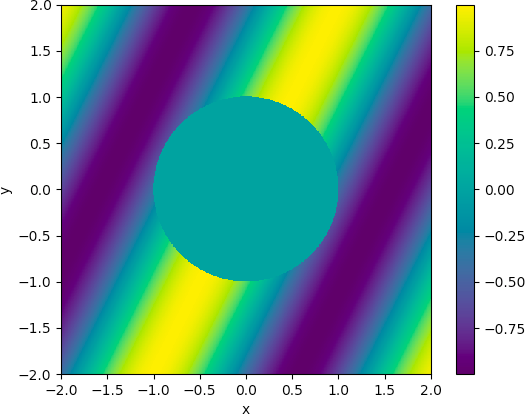
\includegraphics[width=6cm]{../figures/incident_field}\label{fig:incident_field}
\end{figure}

For the scattered field class, there are a few more functions:

\begin{lstlisting}
class ScatteredField(Wave, Inputs):
    def __init__(self):
        print('>>> ScatteredField started...')
        Wave.__init__(self)
        Inputs.__init__(self)

    def get_value_z(self, x, y):
        '''
        Returns the value of Z at a given (x, y).
        '''
        r = self.get_r(x, y)
        if r >= self.get_cylinder_radius():
            return self.get_sum(r, self.get_theta(x, y))
        else:
            return 0

    def get_sum(self, r, theta):
        '''Actions the summation up to the truncation number and
        returns the approximate value for z for a given point.'''
        z = 0   #Initialising
        for n in range(self.truncation):
            z += self.get_constant_term(n) * self.get_angular_term(n, theta) * self.get_radial_term(n, r)
        return z

    def get_constant_term(self, n):
        if self.boundary_type.lower() in 'neumann':
            return self.get_modified_neumann_factor(n) * self.get_neumann_bc(n)
        elif self.boundary_type.lower() in 'dirichlet':
            return self.get_modified_neumann_factor(n) * self.get_dirichlet_bc(n)
        else:
            raise TypeError('Invalid boundary type.')

    def get_angular_term(self, n, theta):
        return np.cos(n*(theta - self.get_incident_angle()))

    def get_radial_term(self, n, r):
        return sp.hankel1(n, self.get_wavenumber()*r)\end{lstlisting}

Here it starts becoming clear why my tool is so slow. The algorithm does not just loop through each coordinate to find a value of $z$, it also loops through the summation up to the truncation number, and it does this for the constant, angular and radial terms. I am sure there is a better, more efficient way to go about this but I have not found it yet.

Finally, we have the \verb!TotalField! classes:
\begin{lstlisting}
class TotalField(Wave, Inputs):
    '''
    TODO: docstring
    '''
    def __init__(self):
        print('>>> TotalField started...')
        Wave.__init__(self)
        Inputs.__init__(self)
        self.incident = IncidentField()
        self.scattered = ScatteredField()

    def get_value_z(self, x, y):
        return self.incident.get_value_z(x, y) + self.scattered.get_value_z(x,y)
\end{lstlisting}

this is what is actually plotted.

\begin{figure}
  \centering
  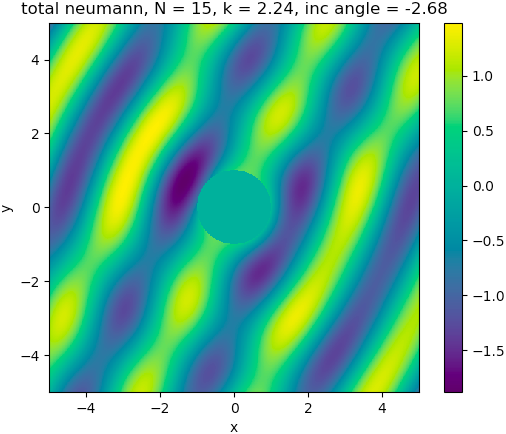
\includegraphics[width=6cm]{../figures/total_neumann_n15}
  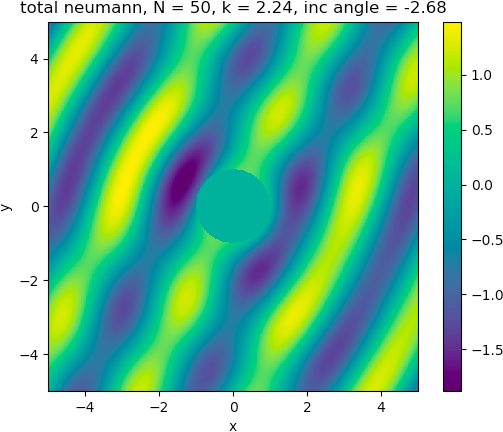
\includegraphics[width=6cm]{../figures/total_neumann_n50}
  \caption{Total field with Neumann BC for N=15 and N=50}
\end{figure}

\begin{figure}
  \centering
  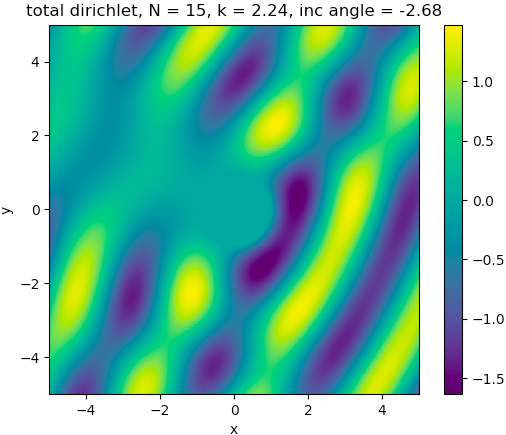
\includegraphics[width=6cm]{../figures/total_dirichlet_n15}
  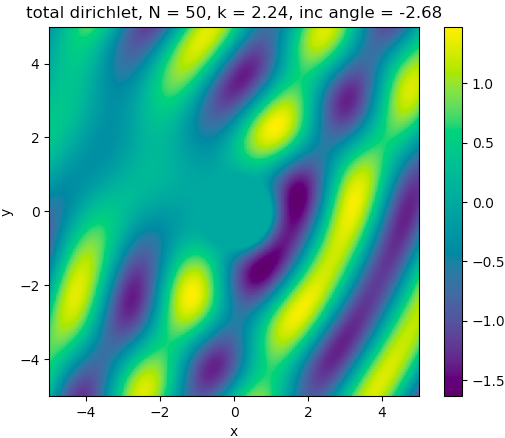
\includegraphics[width=6cm]{../figures/total_dirichlet_n50}
  \caption{Total field with Dirichlet BC for N=15 and N=50}
\end{figure}

\section{Scattering inside the cylinder}

For the transmission problem, I decided to create new methods for the inside of the cylinder, and pull in the methods from the scattered field earlier for the outside, instead of creating new ones for this too. This mean that I had to add a boundary condition for this problem to the \verb!ScatteredField! class. I added an \verb!elif! term in the \verb!get_constant_term! function to make sure I was using the correct constants

\begin{lstlisting}
def get_constant_term(self, n):
    if self.boundary_type.lower() in 'neumann':
        return self.get_modified_neumann_factor(n) * self.get_neumann_bc(n)
    elif self.boundary_type.lower() in 'dirichlet':
        return self.get_modified_neumann_factor(n) * self.get_dirichlet_bc(n)
    elif self.boundary_type.lower() in 'interior':
        return self.get_bc_interior_field(n)
    else:
        raise TypeError('Invalid boundary type.')
\end{lstlisting}

and then created the boundary condition for the transmission problem

\begin{lstlisting}
def get_bc_interior_field(self, n):
    return ((self.density_inside-self.density_outside) * sp.jv(n, self.get_wavenumber() * self.cylinder_radius)* sp.jvp(n, self.get_wavenumber() * self.cylinder_radius,1))/(self.get_radiation_resistance_outside(n)-self.get_radiation_resistance_inside(n))
\end{lstlisting}

The radiation resistance variables are simply $R_1$, $R_2$ in the theory chapter, it makes the code more readable to give them descriptive names instead.

The class itself is constructed in much the same way as the other two.

\begin{lstlisting}
class InteriorField(Wave, Inputs):
    def __init__(self):
        print('>>> InteriorField started...')
        Wave.__init__(self)
        Inputs.__init__(self)
        self.scattered = ScatteredField()
        self.outside = TotalField()

    def get_value_z(self, x, y):
        '''
        Returns the value of Z at a given (x, y).
        '''
        r = self.get_r(x, y)
        theta = self.get_theta(x, y)

        if r <= self.get_cylinder_radius():
            return self.get_sum_inside(r, theta)
        else:
            return self.outside.get_value_z(x,y)

    def get_sum_inside(self, r, theta):
        '''Actions the summation up to the truncation number and
        returns the approximate value for z for a given point.'''
        z = 0   #Initialising
        for n in range(self.truncation):
            z += self.get_constant_term_inside(n) * sp.jv(n, self.get_wavenumber() * r) * np.cos(n*(theta - self.get_incident_angle()))
        return z

    def get_constant_term_inside(self, n):
        return (self.density_inside * self.get_radiation_resistance_outside(n) - self.density_outside * self.get_radiation_resistance_inside(n)) / (self.density_inside * (self.get_radiation_resistance_outside(n)- self.get_radiation_resistance_inside(n)))
\end{lstlisting}

Unfortunately this did not work well at all.

\section{Secondary plots}\label{ss:secondary_plots}
I used python to create the plots in Chapter 2.
%
  \begin{lstlisting}[caption={Plot of bessel functions of integer order},label={lst:bessel_int_no}]
x=np.linspace(0,5,100)

fig=plt.figure()
ax=fig.add_subplot(111)

for n in range(6):
    ax.plot(x,sp.jv(n, x), label=str(n))

plt.axhline(color='black',
            linewidth = 0.5)

plt.legend(loc=1)
plt.title('Bessel function of order n.')
plt.show()\end{lstlisting}\par
%
The code for the Neumann functions plot was similar, replacing \verb!sp.jv(n,x)! on line 7 by \verb!sp.yn(n,x)!. I also had to adjust the axis to make sure we got a meaningful plot, see \figref{fig:neumann_bounding_axis}.\par
%
\begin{figure} \centering
  %
  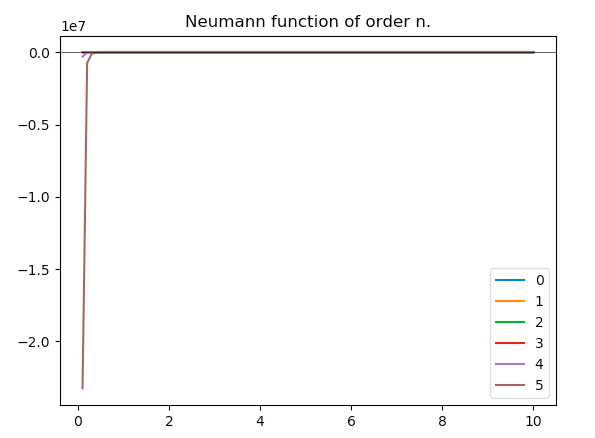
\includegraphics[width=6cm]{../figures/plot_neumann_unbounded_y}
  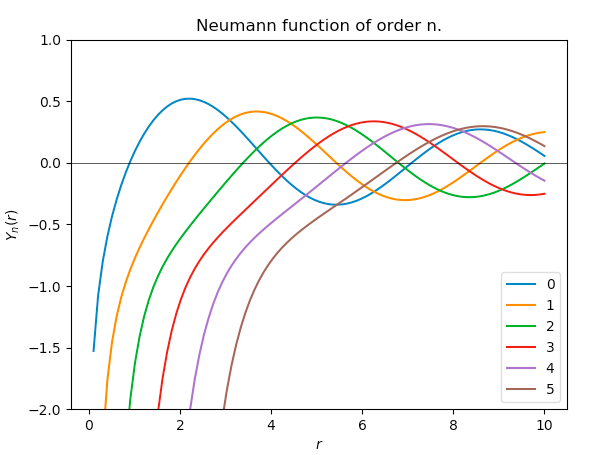
\includegraphics[width=6cm]{../figures/plot_neumann_int_order}
  \caption{Neumann functions with and without bounded axis}\label{fig:neumann_bounding_axis}
  %
\end{figure}
%
\begin{lstlisting}[caption={Plot of neumann functions of integer order},label={lst:neumann_int_no}]
x=np.linspace(0,10,100)

fig=plt.figure()
ax=fig.add_subplot(111)

axes = plt.gca()
axes.set_ylim([-2,1])

for n in range(6):
    ax.plot(x,sp.yn(n, x), label=str(n))

plt.axhline(color='black',
            linewidth = 0.5)

plt.legend(loc=4)
plt.title('Neumann function of order n.')
plt.show()\end{lstlisting}\par
%
For Hankel functions I decided to plot the absolute value. If we do not specify when plotting, \verb!matplotlib! takes the real part of a complex number, so withou the \verb!abs! command this was just plotting a Bessel function.
%
\begin{lstlisting}[caption={Plot of hankel functions of integer order},label={lst:hankel_int_no}]
x=np.linspace(0,7,100)

fig=plt.figure()
ax=fig.add_subplot(111)

axes = plt.gca()
axes.set_ylim([0,4])

for n in range(6):
    ax.plot(x,abs(sp.hankel1(n, x)), label=str(n))

plt.legend(loc=1)
plt.title('Absolute value of the Hankel function of the first type of order n.')
plt.ylabel('$H_{n}^{(1)}(r)$')
plt.xlabel('$r$')
plt.show()\end{lstlisting}\par

\section{Limitations}

In short, this tool was not entirely succesfull. However it was a really valuable learning experience for me. I came into this with \verb!hello world! level understanding of Python, and I now have a grasp of what good object oriented architecture looks like, why it matters and where improvements can be made.

The first and most important improvement, clearly, needs to be accuracy. The code is no use if it cannot produce accurate plots.

Second, is speed. My laptop is not very powerful but even so, some of these plots took a \emph{very long time} to render. I have a rough idea of where the weak points efficiency-wise are, but this wasn't a priority and I couldn't see a clear way to fix them, or patch it up to loose a few minutes off of computing time.

Finally, the structure of the file itself has gone through so many iterations it is not entirely clear or accessible to read. There are a lot of places where functions are defined in classes where they do not belong.
